\begin{question}[section=7,name={Feldbild},difficulty=,quantity=5,type=thr,tags={}]
	Skizziern sie die Feldbilder des TEM-Modus für E und H in einem Koaxialkabel!
	\\ \textbf{Hinweis:}\\
	Siehe Abb. 7.1 u.Skript Seite 78
\end{question}
\begin{solution}
	\begin{figure}[H]
		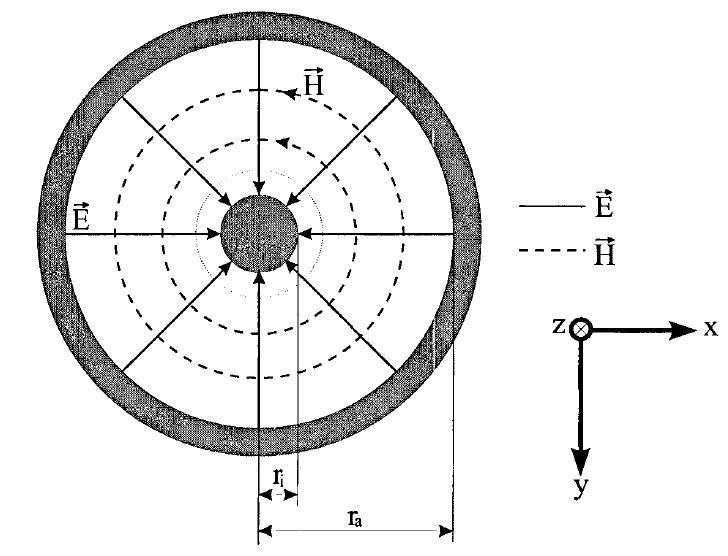
\includegraphics[width=6cm]{./opn/exm/thr/chp/7/1/bild.jpeg}
	\end{figure}
	E-Feld radial nach innen gerichtet, H-Feld konzentrisch um den Innenleiter im Innenraum.
\end{solution}